\documentclass[conference]{IEEEtran}
\usepackage{amsmath,amssymb,amsfonts}
\usepackage[utf8]{inputenc}
\usepackage{url}
\usepackage{subfigure}
\usepackage{booktabs,threeparttable,multirow}
\usepackage{graphicx}
\usepackage{hyperref}

% new math operators
\DeclareMathOperator{\abs}{abs}

% todo command
\usepackage{marginnote}
\newcounter{todocnt}
\setcounter{todocnt}{0}
\newcommand{\todo}[1]{\stepcounter{todocnt}{\tt {[#1]}} \marginpar{{$\blacksquare$ \thetodocnt}}}  
\newcommand{\specialcell}[2][c]{%
  \begin{tabular}[#1]{@{}c@{}}#2\end{tabular}}

\hyphenation{op-tical net-works semi-conduc-tor}
\IEEEoverridecommandlockouts
\begin{document}

\title{Projekt: Rowhammer}


\author{\IEEEauthorblockN{Gilian Henke\\ Dominik Mairhöfer}
\IEEEauthorblockA{University of Lübeck\\
Email: \texttt{gilian.henke@student.uni-luebeck.de}\\ \texttt{dominik.mairhoefer@student.uni-luebeck.de}}}
\maketitle

\begin{abstract}
Das Ziel des Projekts ist es einen One-Location Rowhammer Angriff nach dem Paper \cite{DBLP:journals/corr/abs-1710-00551} zu implementieren. Dieser Angriff soll dann verwendete werden, um lokal die Rechte zu erweitern. Dafür soll unter anderem auch die neue Methode des Memory chasing verwendet werden.\\
Beim hierbei zu Grunde liegenden Modell, kann die Software Schutzmechanismen besitzen, aber nicht die Hardware. Der Angreifer kann ein arbiträres, unprivilegiertes Programm starten. Unter diesen Voraussetzungen kann der Angriff durchgeführt werden.


\end{abstract}

\section{Motivation}
\todo{Know what you want to do and why that is interesting (maybe with bullet points). But do not write this section until you know what you actually have done so that the motivation fits your work. Aus diesen genannten Gründen noch nicht geschrieben.}


We will stick to the following timeline: (Zur Orientierung beibehalten)

\begin{itemize}
	\item 12/18:  Submission of motivation, background, project scope and related work: please give a description of the technical aspect of your work, i.e. detailed background description of attacks. Also describe related work and outline, in more detail, your technical steps.
	\item 1/15: First version of report. This should be ver close to the final version, only technical parts that have not yet been finished should be missing.
	\item 2/1 : Final submission of complete project description.
	\item 2/8: Project Presentations in class: 25 minutes presentation plus questions. 
\end{itemize}

\section{Hintergrund}\label{sec:background}
Die hier betrachteten Rowhammer Angriffe basieren auf folgendem Modell. Das System, auf welchem der Angriff ausgeführt werden soll, besitzt keine Maßnahmen der Hardware, um Rowhammer Angriff zu entdecken und zu unterbinden. Die verwendete Software darf jedoch versuchen, zu erkennen, ob ein Angriff stattfindet, und jenen zu verhindern. Damit solch ein Angriff überhaupt ausgeführt werden kann, muss der Angreifer in der Lage sein, ein beliebiges, nicht privilegiertes Programm auf dem System zu starten.\\
Im Folgendem werden dann die Methoden beschrieben, mit denen ein Rowhammer Angriff ausgeführt werden kann. Im Rahmen dieses Projekts wird dann versucht, einen Teil dieser Methoden anzuwenden und zu implementieren.
\subsection{Überblick über den Angriffsablauf}
Der in dem Paper beschriebene Angriff lässt sich in mehrere einzelne Schritte unterteilen. Diese laufen in der folgenden Reihenfolge ab:
\begin{enumerate}
	\item One-Location Rowhammer \\
	Zuerst wird durch einen One-Location Rowhammer Angriff versucht wahllos Bits im Speicher zu flippen. Dies dient dazu, Adressen im virtuellen Adressbereich zu finden, für die es überhaupt möglich ist Bits zu flippen.
	
	\item Prefetch Side-Channel Attack \\
	Anschließend werden mit Hilfe einer Prefetch Side-Channel Attacke die physikalischen Adressen zu den im ersten Schritt gefundenen virtuellen Adressen herausgefunden.
	
	\item Memory Waylaying \& Prefetch Side-Channel Attack \\
	Um ein Bit in einer Datei zu flippen, für die es keine Schreibrechte gibt, wird diese in den Arbeitsspeicher geladen. Mit Memory Waylaying wird sie immer wieder an unterschiedliche Adressen geladen. Nach jedem neuen Laden wird mit der Prefetch Side-Channel Attacke die physikalische Adresse herausgefunden, an die die Datei geladen wurde.
	Wurde die Datei an eine physikalische Adresse geladen, für die in den ersten beiden Schritten herausgefunden wurde, dass sie für einen One-Location Rowhammer Angriff verwundbar ist, wird mit dem nächsten Schritt fortgefahren.
	
	\item One-Location Rowhammer
	Da die Datei nun an einer bekannten Adresse liegt, kann der  One-Location Rowhammer Angriff aus dem ersten Schritt für diese Adresse erneut ausgeführt werden. Damit wird ein Bit an der physikalischen Adresse geflippt und man erhält eine veränderte Datei.
\end{enumerate}

Im folgenden werden die einzelnen Schritte genauer beschrieben.

\subsection{Memory Waylaying}
In dem Paper werden zwei neue Methoden vorgestellt, um eine Seite an einer bestimmten physikalischen Adresse im Arbeitsspeicher zu platzieren. Dieser Prozess nennt sich Memory Waylaying. Hierbei wird im Gegensatz zu anderen Methoden nicht der gesamte Speicher mit Daten gefüllt, was die Entdeckung schwieriger macht. Das dies möglich ist, beruht darauf, dass, wenn Daten, wenn sie aus dem DRAM entfernt werden, beim Laden an eine zufällige Adresse platziert werden. Durch wiederholtes Anwenden dieser Methode kann die Seite an die richtige Position im Speicher positioniert werden.\\
 Mit Hilfe eines Prefatch-based Prediction Oracle, näher beschrieben in \cite{DBLP:conf/ccs/2016}, kann dann überprüft werden, ob zwei virtuelle Adressen, auf die gleiche physikalische verweisen. Damit kann dann überprüft werden, ob eine Seite an einer bestimmten Stelle im Speicher liegt. Dieses Orakel besteht aus zwei Schritten. Zunächst der prefatch und dann eine Flush and Reload Attacke. \\
Da der komplette Prozess des Memory Waylaying Laufzeiten von 100 Stunden benötigt. werden wir die effizientere Variante des Memory Chasing betrachten und implementieren. Beim Memory Chasing wird der copy-on-write Efekt des \textit{fork}-Befehls ausgenutzt.
\subsection{One-Location Rowhammer}
Durch die fortschreitende Entwicklung vom DRAM, werden einzelne Speicherzellen mit immer weniger Spannung betrieben. Dies führt jedoch, dazu dass schon geringe Änderungen der Spannung ein Flip eines Bits zur Folge haben können. Dieses Flippen kann man durchs gehäufte, schnelle Zugreifen auf benachbarte Speicherzellen, Hämmern genannt, bewusst auslösen.
 Beim double-sided Rowhammer wird auf beiden Seiten der zu flippenden Speicherreihen gehämmert, während beim single-sided Rowhammer nur eine Seite gehämmert wird. Im Gegensatz zum Namen wird bei diesen Angriffen jedoch mehr als nur eine einzige Speicherzelle gehämmert.\\
Betrachten wir als nächstes den One-Location Rowhammer. Bei dieser Methode wird im Gegensatz zu den üblichen Methoden nur eine einzige Stelle im Speicher gehämmert und dann überprüft, ob im benachbarten Speicher Bitflips aufgetreten sind. Hierbei werden zwar weniger Bitflips erzeugt, aber die Entdeckung ist wesentlich schwieriger. Die Anzahl der hierbei erzeugten Bitflips ist aber immer noch ausreichend, um einen Angriff durchzuführen.\\
Bei der Durchführung dieses Angriffes wird zunächst der zu testende Speicher allokiert und mit zufälligen aber wiedererkennbaren Werten gefüllt. Dann wird durch wiederholtes Hämmern versucht in diesem Speicher ein Bitflip zu erzeugen. Der Einfachheit halber wird bei diesem Angriff immer eine zufällige Adresse gehämmert. Hierbei wird eine Adresse aus dem betrachtetem Speicher zufällig gewählt und dann wird auf jene Adresse wiederholt zugegriffen. Nach jedem Zugriff wird der Wert dieser Adresse jedoch immer wieder aus dem Cache entfernt, zum Beispiel mit \texttt{clflush}, sodass erneut auf den DRAM zugegriffen werden muss. Danach wird überprüft, ob das Hämmern an dieser Adresse irgendeine Veränderung erzeugt hat. Wenn dies eine Veränderung bewirkt hat, dann haben wir unsere Adresse für den Bitflip gefunden. Wenn diese keine Veränderung bewirkt hat, dann wiederholen wir das Hämmern an einer neuen Adresse.\\
Der Vorteil dieses Angriffes gegenüber des double-sided Rowhammer ist, dass er äußerst einfach ist und schwer von herkömmlichen Strategien zu entdecken ist. Der Nachteil hierbei ist es jedoch, dass die Wahrscheinlichkeit für einen Bitflip deutlich geringer ist. Ein weiterer Nachteil ist es, dass man hiermit noch nicht die tatsächliche physikalische Adresse des zu flippenden Speichers erhält, sondern nur dessen virtuelle Adresse.

\subsection{Prefetch Side-Channel Attacke}

Die Prefetch Side-Channel Attacke aus \cite{DBLP:conf/ccs/2016} dient dazu, zu einer virtuellen Adresse die dazugehörige physikalische Adresse herauszufinden. 

Der virtuellen Adressraum jedes Prozesses ist unterteilt in zwei Bereiche. Den User und Kernel Bereich. Ein laufender Prozess im User Modus kann lediglich auf den User Bereich zugreifen und im Kernel Bereich weder lesen noch schreiben. Dies ist nur möglich wenn die CPU im Kernel-Modus läuft und somit dem Kernel vorbehalten. Trotzdem ist auch der Kernel Bereich im virtuellen Adressraum jedes Prozesses enthalten.

Bei einigen Betriebssystemen, insbesondere beim Linux Kernel \cite{virtual-momory}, findet sich im Kernel Bereich eine Region in welcher der gesamte physikalische Speicher in den virtuellen Adressraum gemappt wird.
Zum Beispiel befindet sich beim Linux Kernel diese Region im virtuellen Adressbereich von \texttt{0xffff880000000000} bis \texttt{0xffffc7ffffffffff}.
Das bedeutet auf die physikalische Adresse \texttt{0x00} kann über die virtuelle Adresse \texttt{0xffff880000000000} zugegriffen werden.

Weiter bedeutet dies auch, dass für jede physikalische Adresse, die über eine virtuelle Adresse aus dem User Bereich angesprochen werden kann, eine weitere virtuelle Adresse im Kernel Bereich existiert, die auf die gleiche physikalische Adresse zeigt. Dies ist in Abbildung \ref{fig:direct-mapping} dargestellt.

\begin{figure}
	\centering
	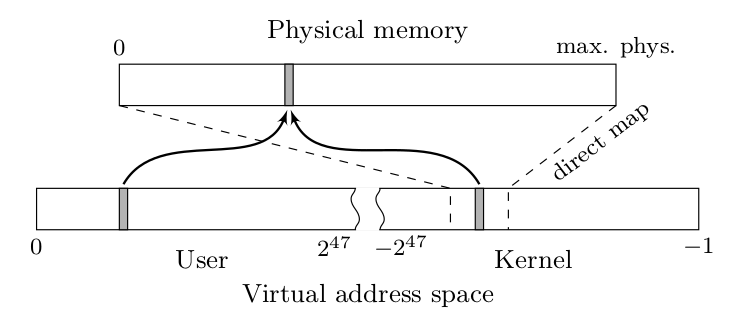
\includegraphics[width=1\linewidth]{direct-mapping}
	\caption{Direktes Mapping des gesammten physikalischen Speichers. Jede pyhsikalische Adresse ist zwei mal vorhanden, einmal im User und Kernel Bereich \cite{DBLP:conf/ccs/2016}}
	\label{fig:direct-mapping}
\end{figure}


Ist für eine virtuelle Adresse aus dem User Bereich die dazugehörige virtuelle Adresse aus dem Kernel Bereich bekannt, lässt sich offensichtlich die physikalische Adresse einfach berechnen, indem von der virtuellen Adresse im Kernel Bereich der Offset \texttt{0xffff880000000000} abgezogen wird. Die Schwierigkeit liegt darin, diese Adresse zu finden. 


Um die passende virtuelle Adresse im Kernel Bereich zu finden kann nun folgende Eigenschaft ausgenutzt werden:

Auf modernen Prozessoren gibt es einen \texttt{prefetch} Befehl, welche die CPU darauf hinweist, dass die Daten unter einer bestimmten Adresse bald benötigt werden. Die CPU lädt diese dann in den Cache, damit sie schneller verfügbar sind. Entscheidend dabei ist, dass man jede Adresse aus dem virtuellen Adressbereich mittels \texttt{prefetch} in den Cache laden kann, auch solche die im Kernel Bereich liegen. Der Cache der CPU beruht jedoch auf physikalischen Adressen. Das bedeutet, wenn eine Adresse in den Cache geladen wird, wird bei jedem zugriff auf eine virtuelle Adresse die auf die physikalische zeigt, auf den Cache zugegriffen.

Mithilfe des prefetchings kann nun eine Cache Timing Attacke durchgeführt werden, welche wie folgt abläuft:
\begin{enumerate}
	\item Auf die virtuelle Adresse im User Bereich, zu welche die dazugehörige im Kernel Bereich gefunden werden soll, wird ein \texttt{flush} ausgeführt. Dadurch wird diese aus allen Caches der CPU entfernt. 
	\item Anschließend wird eine virtuelle Adresse aus dem Kernel Bereich mittels eines \texttt{prefetch} in den Cache geladen.
	\item Dann wird lesen auf die Adresse aus dem User Bereich zugegriffen. Erfolgt der Lesezugriff schnell, wurde die Adresse wahrscheinlich zwischendurch in den Cache geladen und die virtuellen Adressen aus User und Kernel Bereich zeigen aus die gleiche physikalische Adresse. Erfolgt der Zugriff langsam ist dies wahrscheinlich nicht der Fall.
\end{enumerate}

Diese Schritte können nun für alle virtuellen Adressen von texttt{0xffff880000000000} bis \texttt{0xffffc7ffffffffff} wiederholt werden, bis einmal ein schneller Zugriff erfolgt und somit die passende Adresse aus dem Kernel Bereich gefunden wurde.

Um zuverlässig ein korrektes Ergebnis zu erhalten muss im dritten Schritt sehr hochauflösend die Zeit gemessen werden. Dies kann mit Hilfe des \texttt{rdtsc} Befehls erfolgen, mit dem die Anzahl an Clock-Zyklen der CPU gemessen werden können. Nach \cite{DBLP:conf/ccs/2016} liegt die Anzahl der Zyklen bei einem Zugriff auf Cache bei circa 180, und ansonsten bei circa 380.
Weiter muss die Messung für jede zu prüfende Adresse aus dem Kernel Bereich sehr oft durchgeführt werden, da der \texttt{prefetch} Befehl nicht zuverlässig ist. Er weißt die CPU lediglich darauf hin die Daten in den Cache zu laden, die Entscheidung ob dies wirklich erfolgt liegt jedoch bei der CPU.

Wurde die passende Adresse im Kernel Bereich gefunden lässt sich anschließend wie oben beschrieben die physikalische daraus ableiten. 
% TODO code



\subsection{Privilege Escalation Attacke}
Mit den beschriebenen Methoden lassen sich zwei Arten von Angriffen durchführen: Eine Privilege Escalation Attacke oder eine Denial-of-Service Attacke. In diesem Projekt verwenden wir die Methoden, um eine Privilege Escalation Attacke durchzuführen und dadurch Root-Rechte auf dem System zu erhalten.



\subsection{Abgrenzung des Themas}
Im folgenden gehen wir auf Themen ein, welche zwar im Paper angesprochen werden, wir im Rahmen dieses Projektes jedoch nicht weiter betrachten werden.
\subsubsection{Intel SGX}
Intel SGX (Software Guard Extension) ist eine Erweiterung, um Speicherbereich vor anderen Prozessren, insbesondere auch privilegierten, zu beschützen. Dadurch sollen Angriffe schlechter erkannt werden. Diese Erweiterung ist jedoch nicht auf jedem Rechner vorhanden. Außerdem ist sie nicht zwingend notwendig, One-Location Rowhammer Angriff durchzuführen. Daher werden wir die Verwendung dessen nicht weiter betrachten.
\subsubsection{Memory Waylaying}
Die erste der im Paper bechriebenen Methoden zum Memory Waylaying, hat zu lange Laufzeiten, als das sie im Rahmen dieses Projekts vernünftig untersucht werden kann. Dementsprechend werden wir jene nicht implementieren.
\subsubsection{Denial-of-Service Attacke}
Die hier beschrieben Denial-of-Service Attacke benötigt Intel SGX und wird dementsprechend von uns nicht weiter betrachtet.
\subsection{Weitergehende Arbeiten}
In \cite{seaborn2015} werden die Angriff in leicht verständlicher Art anschaulich dargestellt und geben einen Ansatz, um eine Implementation selbst durchzuführen.\\
In \cite{vanderVeen:2016:DDR:2976749.2978406} wird eine deterministische Version des Angriffs auf Android-Systeme und eine Verallgemeinerung dieses Angriffes auf Linux-Systeme vorgestellt.



\section{Work Description}
Here you describe the work you have performed, problems you have solved and methods you have used. There is a fine balance between brevity and conciseness and ensuring that other people, if investing the time, would be able to reproduce your results given this description.
\todo{this}


\section{Results}
\todo{here you will present and discuss your outcomes: implementation results or measurements or other project outcomes}

\section{Conclusion}
\todo{TBD last}



\bibliographystyle{IEEEtran}
%\bibliographystyle{IEEETR}
\bibliography{verzeichnis1}{}
%\bibliographystyle{abbrv}
\end{document}
